\documentclass{beamer}
\usetheme{Madrid}

\usepackage[utf8]{inputenc}
\usepackage{graphicx}
\usepackage{hyperref}
\usepackage{color}
\usepackage{natbib}
\usepackage{aastex-compat}
\usepackage{siunitx}
\usepackage{aas_macros}
\usepackage{amsmath}
\title[PhD Thesis]{Estudio de la Interacción de Flujos Múltiples de Fuentes Astrofísicas, Aplicada a los Proplyds Clásicos de la Nebulosa de Orión}
\author[M.C Jorge Alejandro Tarango Yong]{Presents: M.C Jorge Alejandro Tarango Yong \\
  PhD Advisor: Dr. William Henney \\
  Tutorial Committee: Dr. Javier Ballesteros, Dr. Luis Zapata}
\date{\today}
\definecolor{AZUL}{HTML}{000032}
\definecolor{DORADO}{HTML}{A87A00}
\setbeamercolor{title}{fg=AZUL, bg=DORADO}
\setbeamercolor{frametitle}{fg=AZUL, bg=DORADO}
\setbeamercolor{structure}{fg=AZUL, bg=DORADO}
\setbeamertemplate{enumerate items}[square]
\setbeamertemplate{section in toc}[square]
\newcommand\thC{\(\theta^1\)\,Ori~C}
\newcommand\Ion[2]{\ensuremath{\mathrm{#1\,\scriptstyle #2}}} %Used when naming different ions. Credit: William J. Henney
\newcommand{\twocols}[2]{
  \begin{columns}
    \begin{column}{5.8cm}
      #1
    \end{column}
    \begin{column}{5.8cm}
      #2
    \end{column}
  \end{columns} 
}

\newcommand{\twocolspic}[2]{
  \begin{columns}
    \begin{column}{4.2cm}
      #1
    \end{column}
    \begin{column}{7.6cm}
      #2
    \end{column}
  \end{columns} 
}

\begin{document}
\frame{\frametitle{PhD Thesis Defense}
  
\includegraphics[scale=0.1]{../Figures/logo}
  \maketitle}

\frame{\frametitle{Index}
  \tableofcontents}
\section{Introduction}
\frame{\frametitle{Motivation of this work}
  \twocols{\begin{block}{}
      Bow shocks occur in many kinds of astrophysical scenarios, from galactic to planetary scales. In this work we develop a mathematical tool for characterizing cylindrically symmetric, geometrically thin and optically thin bow shocks based into their geometrical shape and how is oriented respect the plane of sky.
    \end{block}}{\begin{block}{}
      \begin{center}
        \includegraphics[width=0.6\linewidth]{../Figures/collage}
      \end{center}
    \end{block}}
}

\frame{
  \begin{block}{We called it the $\Lambda'-\Pi'$ diagram \citep{Tarango-Yong:2018a}.}
    \begin{center}
      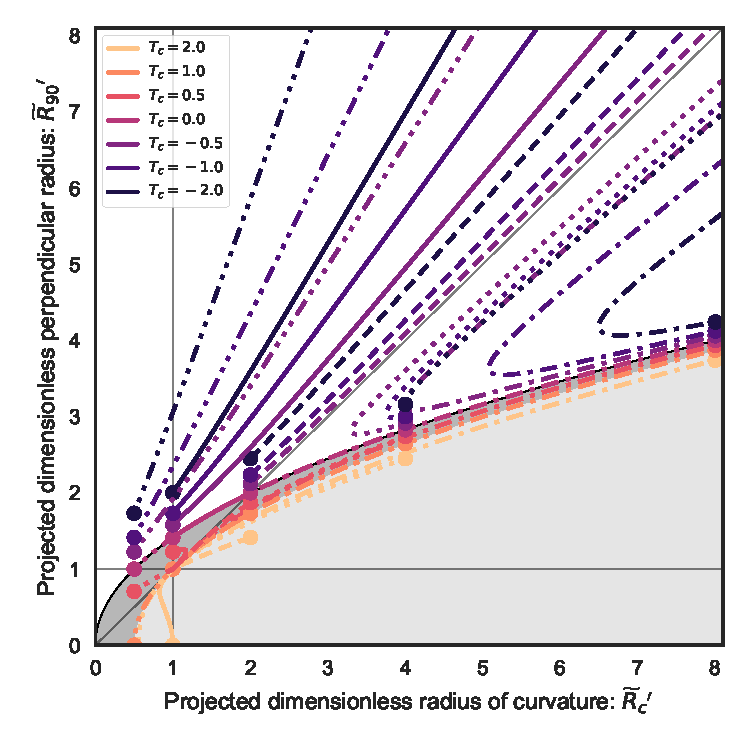
\includegraphics[width=0.6\linewidth]{../Figures/projected-R90-vs-Rc}
    \end{center}
    
    \end{block}
 }
\frame{
  \twocols{\begin{block}{}{
Then we apply this tool to the simplest mathematical surfaces: the quadrics of revolution \citep{Goldman:1983a, Gfrerrer:2009a} and to a simple model for winds interaction: the Thin Shell Model \citep{Canto:1996}.
      }\end{block}}{\begin{block}{}{
        \includegraphics<1>[width=\linewidth]{../Figures/collage2}
        \includegraphics<2>[width=\linewidth]{../Figures/ancantoid-R90-vs-Rc-a}
      }\end{block}}
}
\frame{
  \twocols{\begin{block}{}
      And finally compare the thin shell model against observations of the classical proplyds of the Trapezium in the core of the Orion Nebula in a similar diagram.
    \end{block}}{\begin{block}{}
      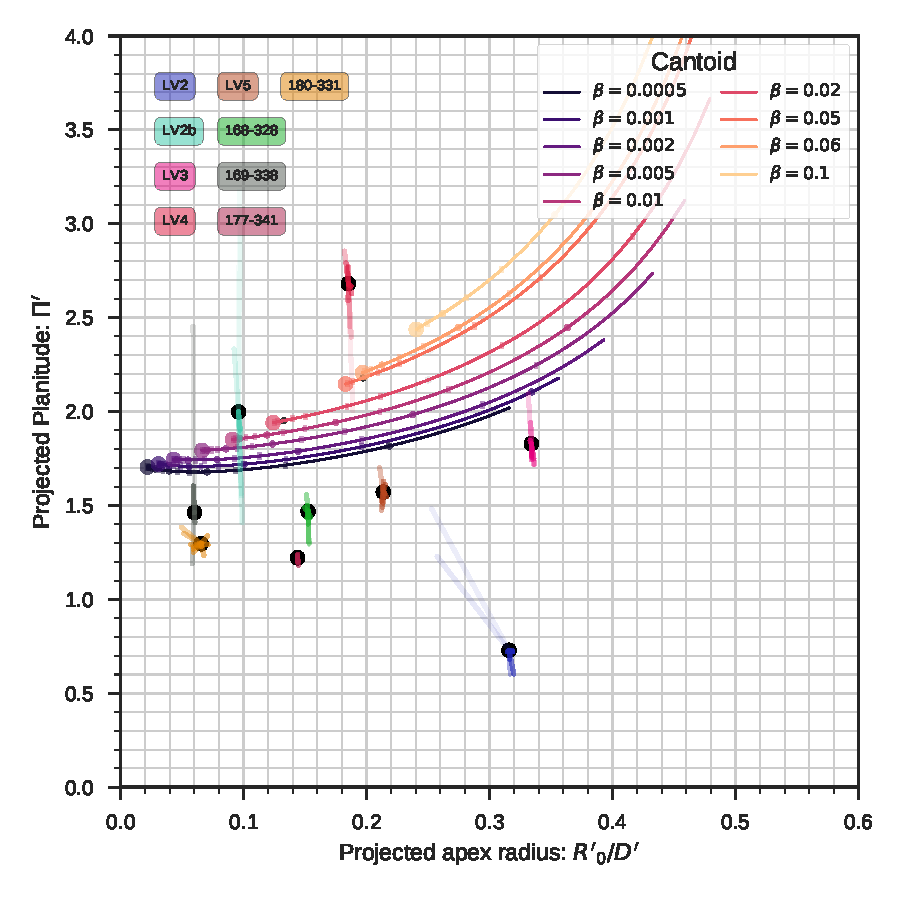
\includegraphics[width=\linewidth]{../Figures/obs-diagnostic-Pi-R0-Cantoid}
    \end{block}}
}
\section{Bow Shocks in the ISM}
\frame{\frametitle{Bow Shocks in the ISM}
  \twocols{\begin{block}{}
      Bow shocks are emmision arcs produced when some fluid interacts at supersonic speeds with another object. Some astrophysical examples seen in the Interstellar Medium (ISM) are:
      \begin{itemize}
      \item \textbf{Jets Surface Work}
      \item Magnetosphere interaction with stellar wind
      \item Stellar Bow shocks
        \begin{itemize}
        \item AGB stars and red supergiants
        \item Runaway O stars
        \item Proplyds
        \item T Tauri stars
        \item Neutron stars
        \end{itemize}
      \end{itemize}
    \end{block}}{\begin{block}{}
      \includegraphics[width=\linewidth]{../Figures/CygnusA} \\
      \footnotesize Cygnus A \citep{Perley:1984}\end{block}
    }
  }

\frame{\frametitle{Bow Shocks in the ISM}
  \twocols{\begin{block}{}
      Bow shocks are emmision arcs produced when some fluid interacts at supersonic speeds with another object. Some astrophysical examples seen in the Interstellar Medium (ISM) are:
      \begin{itemize}
      \item Jets Surface Work
      \item \textbf{Magnetosphere interaction with stellar wind}
      \item Stellar Bow shocks
        \begin{itemize}
        \item AGB stars and red supergiants
        \item Runaway O stars
        \item Proplyds
        \item T Tauri stars
        \item Neutron stars
        \end{itemize}
      \end{itemize}
    \end{block}}{\begin{block}{}
      \includegraphics[width=\linewidth]{../Figures/HJ-Yates}\\
      \footnotesize Density of material flowing from a Hot Jupiter through magnetosphere interacting with stellar wind \citep{Yates:2018}.\end{block}
    }
  }

\frame{\frametitle{Bow Shocks in the ISM}
  \twocols{\begin{block}{}
      Bow shocks are emmision arcs produced when some fluid interacts at supersonic speeds with another object. Some astrophysical examples seen in the Interstellar Medium (ISM) are:
      \begin{itemize}
      \item Jets Surface Work
      \item Magnetosphere interaction with stellar wind
      \item Stellar Bow shocks
        \begin{itemize}
        \item \textbf{AGB stars and red supergiants}
        \item Runaway O stars
        \item Proplyds
        \item T Tauri stars
        \item Neutron stars
        \end{itemize}
      \end{itemize}
    \end{block}}{\begin{block}{}
      \includegraphics[width=\linewidth]{../Figures/cox-betelgeuse}\\
      \footnotesize Observation of a ``Fermata'' type bow shock at \SI{70}{\mu.m} produced by the interaction of the strong wind of a red supergiant ($\alpha$\,Ori) with the ISM \citep{Cox:2012}.\end{block}
    }
  }

\frame{\frametitle{Bow Shocks in the ISM}
  \twocols{\begin{block}{}
      Bow shocks are emmision arcs produced when some fluid interacts at supersonic speeds with another object. Some astrophysical examples seen in the Interstellar Medium (ISM) are:
      \begin{itemize}
      \item Jets Surface Work
      \item Magnetosphere interaction with stellar wind
      \item Stellar Bow shocks
        \begin{itemize}
        \item AGB stars and red supergiants
        \item \textbf{Runaway O stars}
        \item Proplyds
        \item T Tauri stars
        \item Neutron stars
        \end{itemize}
      \end{itemize}
    \end{block}}{\begin{block}{}
      \begin{center} 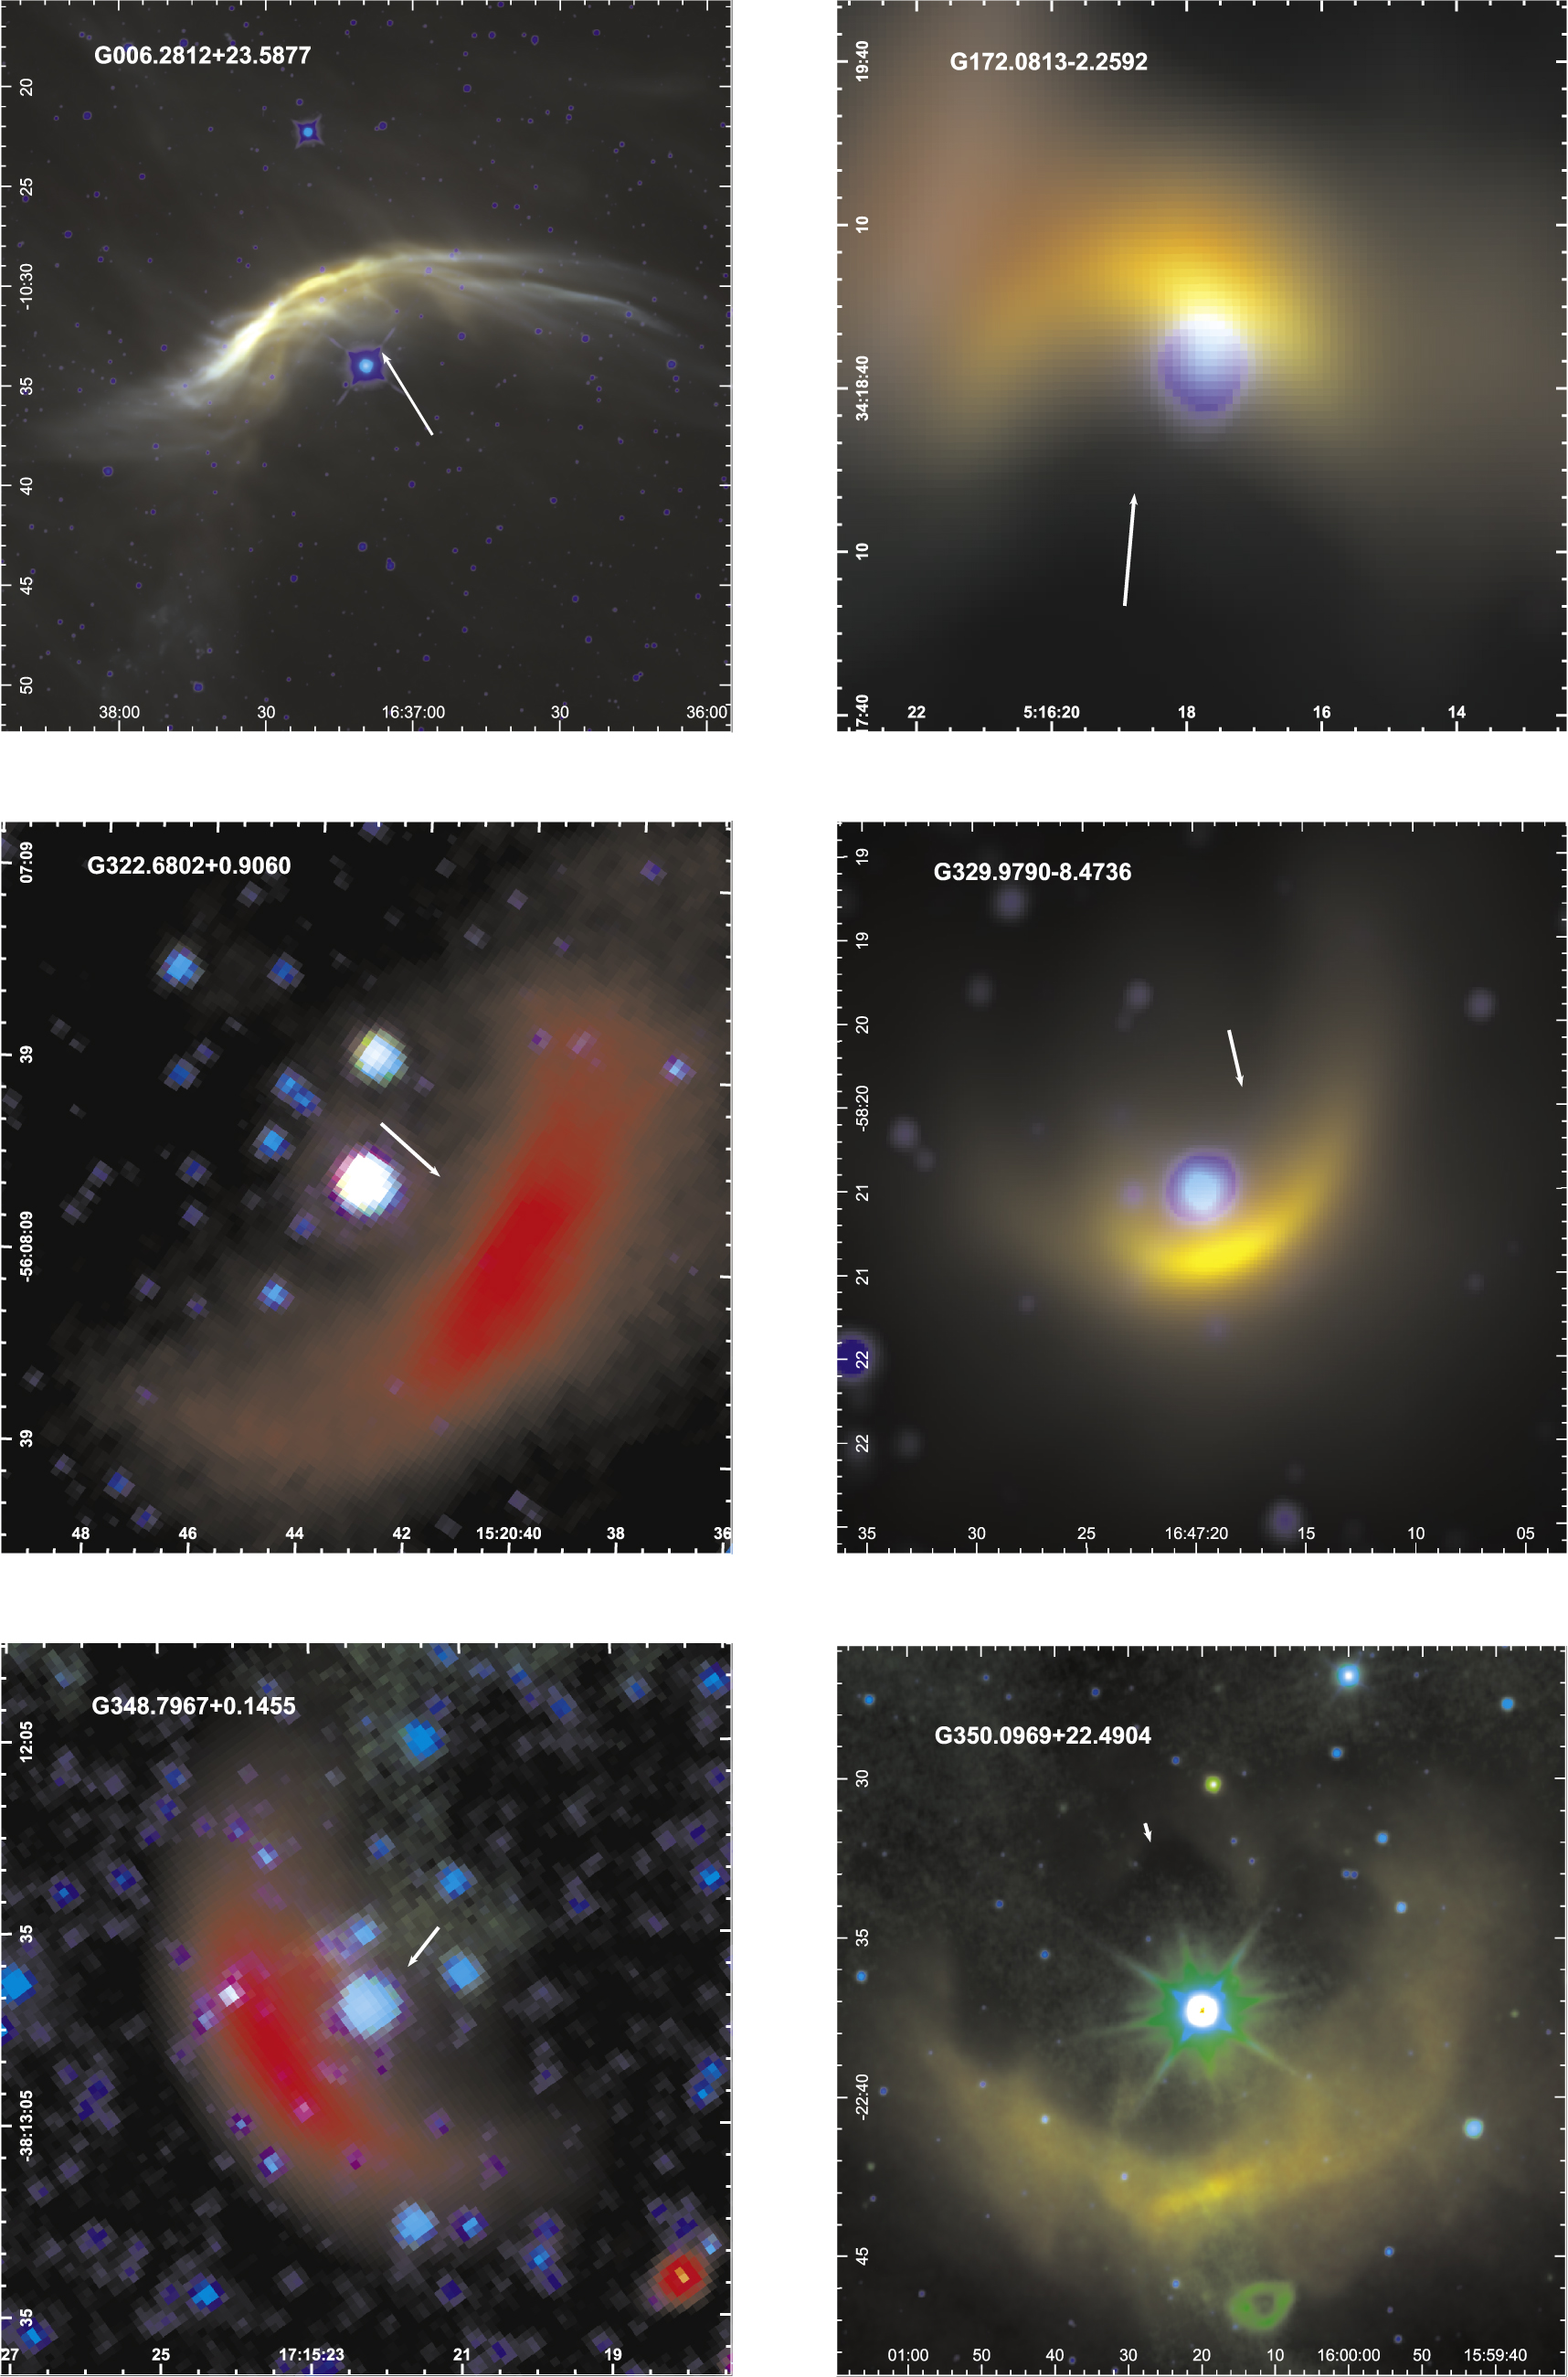
\includegraphics[width=0.5\linewidth]{../Figures/kobulnicky}\end{center}\\
       \footnotesize Observations of prototypical examples of ``Bow shock nebulae'' by Spitzer or WISE produced by runaway stars interacting with the ISM (red: 20 or \SI{22}{\mu.m}, green:8 or \SI{12}{\mu.m}, blue: \SI{4.5}{\mu.m})\citep{Kobulnicky:2016}.\end{block}
    }
  }
  
\frame[label=bally]{\frametitle{Bow Shocks in the ISM}
  \twocols{\begin{block}{}
      Bow shocks are emmision arcs produced when some fluid interacts at supersonic speeds with another object. Some astrophysical examples seen in the Interstellar Medium (ISM) are:
      \begin{itemize}
      \item Jets Surface Work
      \item Magnetosphere interaction with stellar wind
      \item Stellar Bow shocks
        \begin{itemize}
        \item AGB stars and red supergiants
        \item Runaway O stars
        \item \textbf{Proplyds}
        \item T Tauri stars
        \item Neutron stars
        \end{itemize}
      \end{itemize}
    \end{block}}{\begin{block}{}
      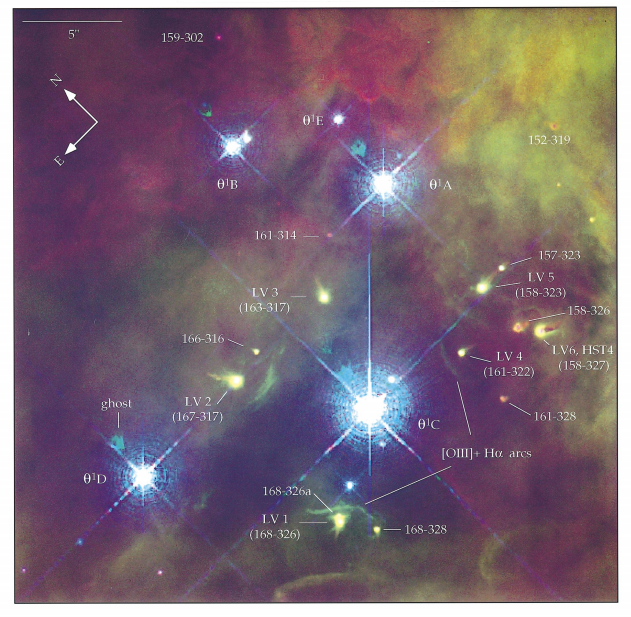
\includegraphics[width=\linewidth]{../Figures/bally-trapezium}\\
     \footnotesize  The Classical proplyds in the core of the trapezium in Orion Nebula also show a bow shock by the HST (red is [\Ion{N}{II}], green is \Ion{H}{\alpha} and blue is [\Ion{O}{I}]) \citep{Bally:1998}.\end{block}}
}
\section{Orion Nebula}
\frame{\frametitle{Orion Nebula}
  \twocols{\begin{block}{}
      The Orion Nebula is the nearest \Ion{H}{II} region ($\sim \SI{414}{pc}$, \citet{Menten:2007}), where massive star formation can be studied with high resolution observations.
    \end{block}}{\begin{block}{}
      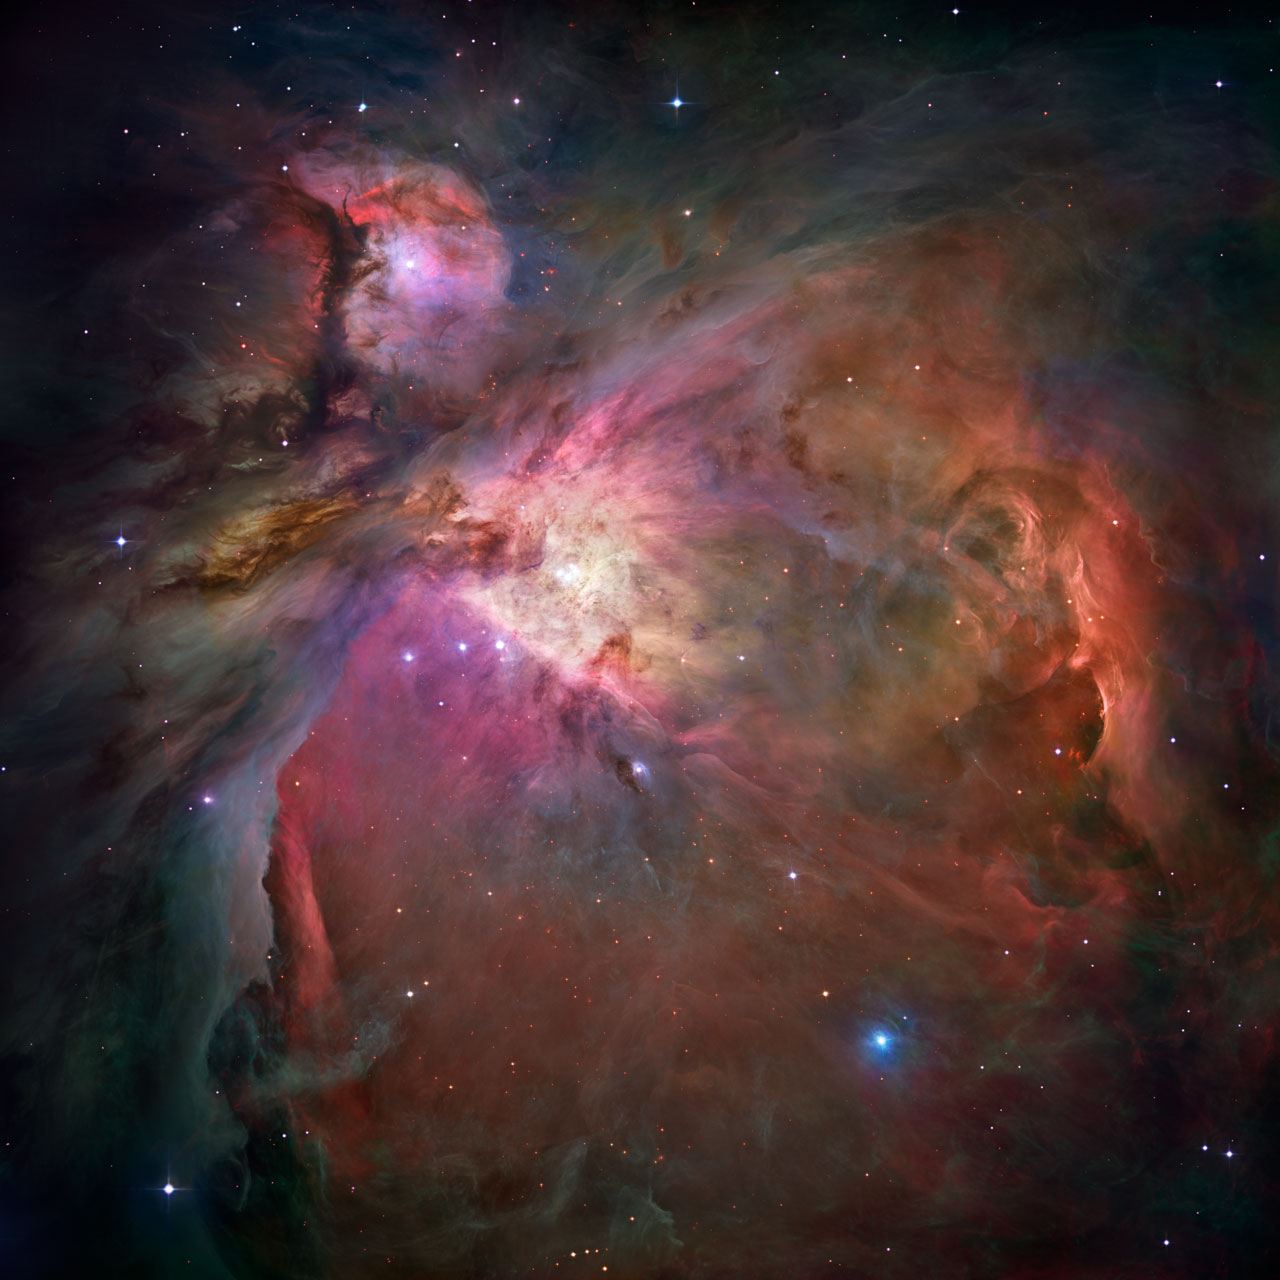
\includegraphics[width=\linewidth]{../Figures/ONC-HST} \\
      www.hubblesite.org
    \end{block}}
}
\frame{\frametitle{Proplyds in Orion Nebula}
  \twocols{\begin{block}{}About 70 arcs have been detected within Orion Nebula \citep{Gutierrez-Soto:2015a}, many of them are produced by proplyds.\end{block}}{\begin{block}{}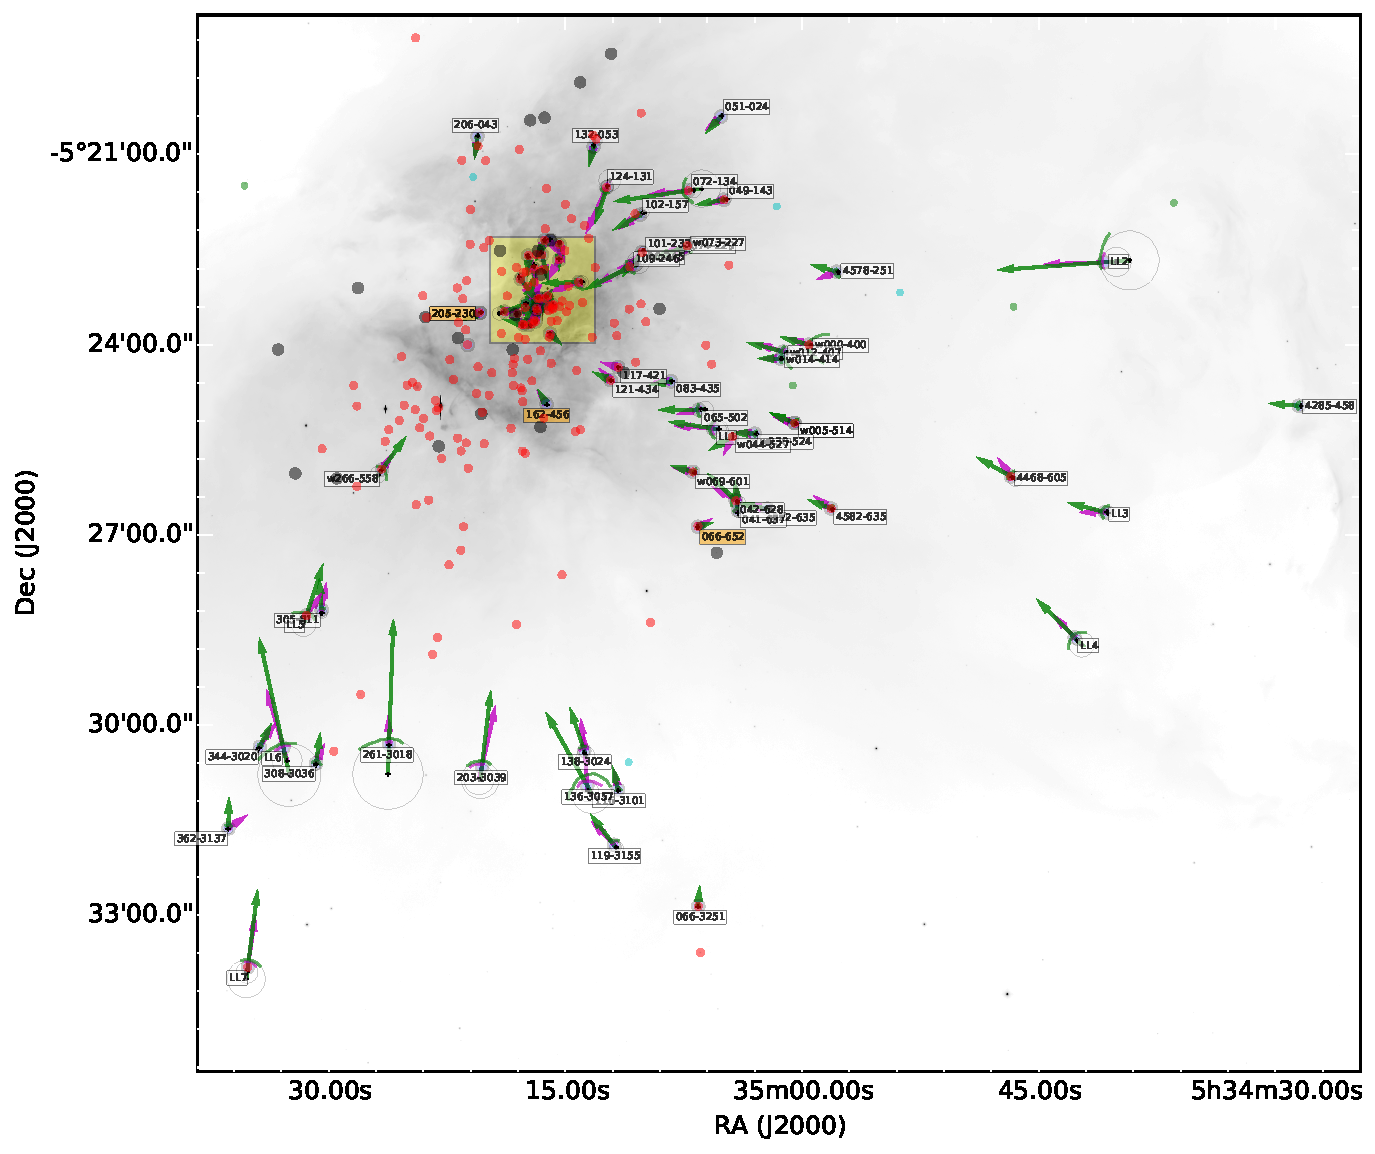
\includegraphics[width=\linewidth]{../Figures/ll-pos-image-Luis} \\
    \footnotesize  Map of bow shocks in Orion Nebula \citep{Gutierrez-Soto:2015a}
    \end{block}}
}

\frame{\frametitle{Proplyds in Orion Nebula}
  \twocols{\begin{block}{}About 70 arcs have been detected within Orion Nebula \citep{Gutierrez-Soto:2015a}, many of them are produced by proplyds.\end{block}}{\begin{block}{}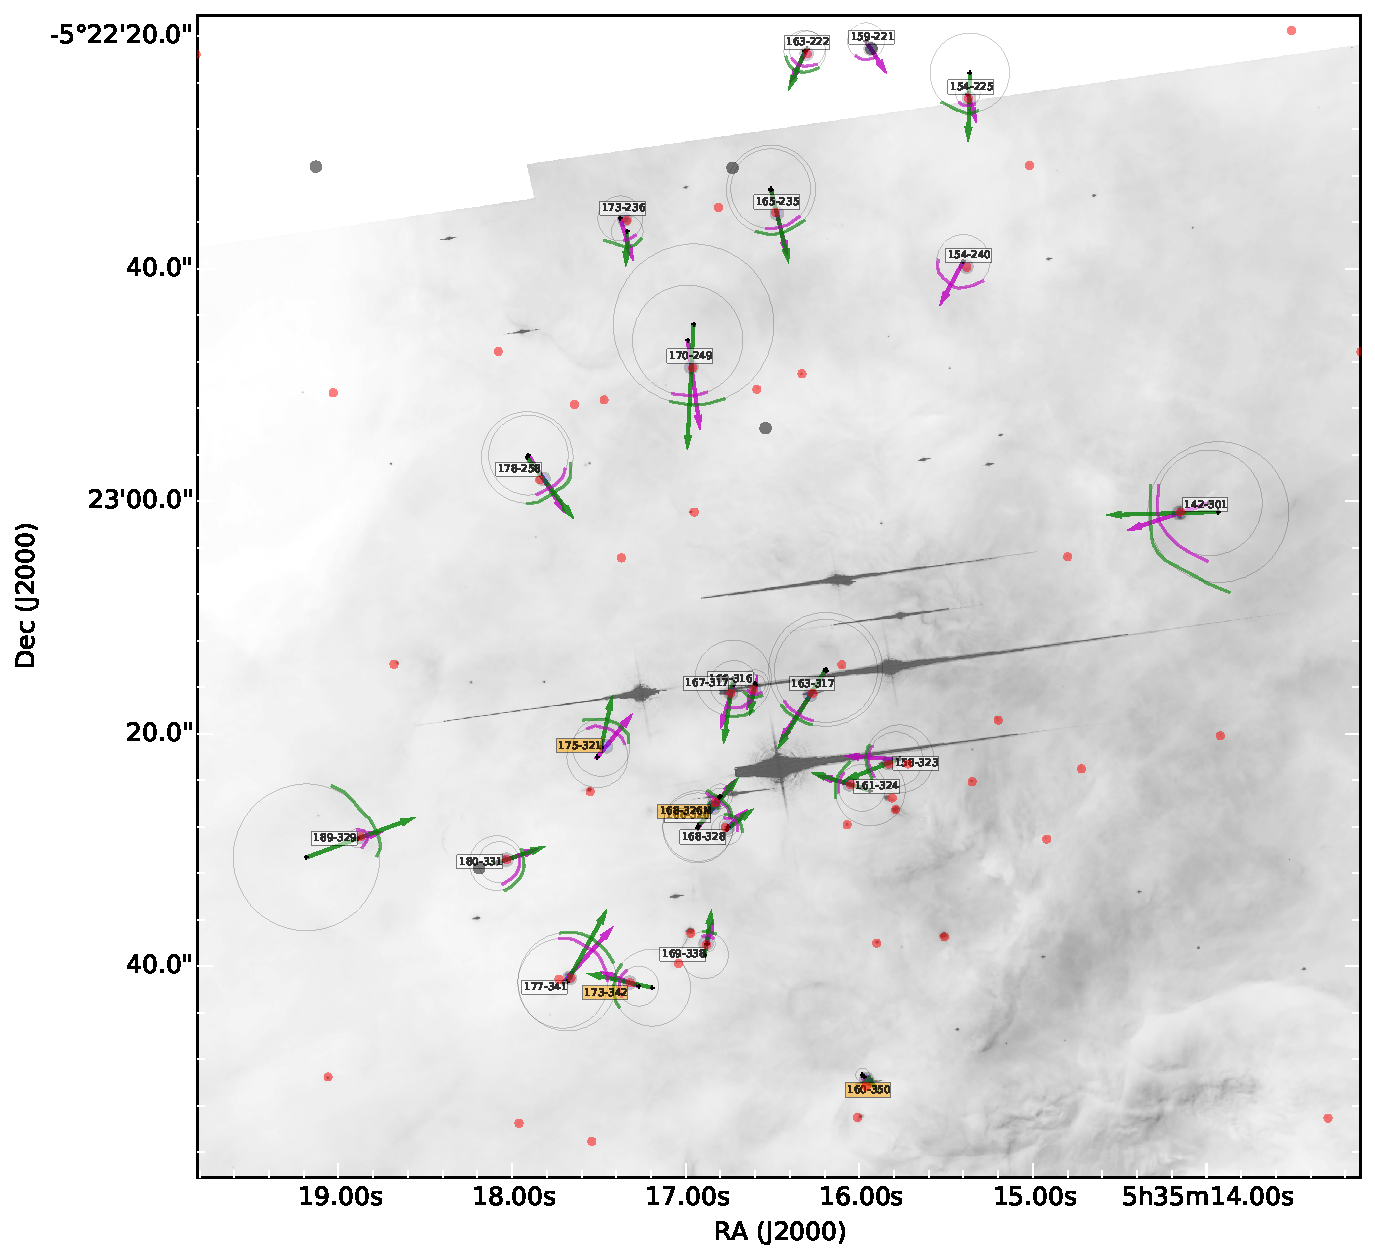
\includegraphics[width=\linewidth]{../Figures/ll-pos-image-zoom-Luis} \\
    \footnotesize  Map of bow shocks in Orion Nebula (Trapezium zoomed) \citep{Gutierrez-Soto:2015a}
    \end{block}}
}

\frame{
  \twocols{\begin{block}{}
      Some of the nearest proplyds to \thC{} were previously observed by \citet{Bally:1998} (slide \hyperlink{bally}{\beamergotobutton{10}}) and \citet{Robberto:2005} in mid infrared and their shape analyzed using the Thin Shell Model from \citep{Canto:1996}, but some proplyds don't fit at all.
    \end{block}}{\begin{block}{}
      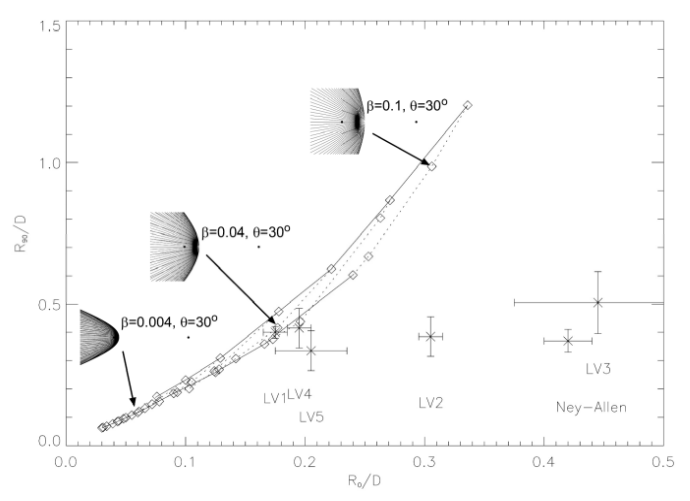
\includegraphics[width=\linewidth]{../Figures/robberto} \\
      \footnotesize Apparent shape of some proplyds (in black points) compared with the thin shell model of \citep{Canto:1996} (open dots and lines) in a $R_{90}/D$ vs $R_0/D$ diagram \citep{Robberto:2005}.
    \end{block}}
}
\frame[label=k-index]{
  
  \begin{block}{}
    \begin{center}
      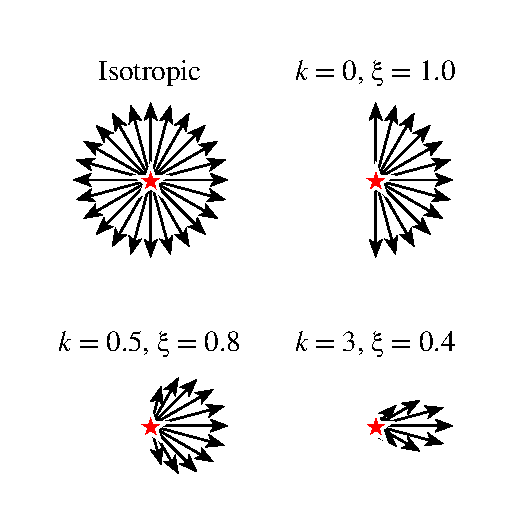
\includegraphics[width=0.5\linewidth]{../Figures/anisotropic-arrows}
      \end{center} \\
      \footnotesize This motivated us to extend \citet{Canto:1996} model to include non isotropic winds.
    \end{block}
}
\frame{\frametitle{Photoevaporated wind in proplyds}
  \twocols{\begin{block}{}
      Proplyds are bright structures with cometary shape which are the result of the photoevaporation of a protoplanetary disk (hence the name) due to a strong source of ultraviolet radiation (e.g a massive star).
    \end{block}}{\begin{block}{}
      \begin{center}
        \includegraphics[width=0.6\linewidth]{../Figures/HST10}
        \end{center} \\
      \footnotesize HST10 is the archetypical example of a proplyd. Image taken with the HST (red: F656N filter, green: F658N, blue: F631N filter, \citet{Tsamis:2013}).
    \end{block}}
}

\frame{
  \twocols{\begin{block}{}
      The incident UV radiation photoevaporates the gas in the protoplanetary disk, which becomes a spherical flow due to pressure gradients. Only the gas located at $r > r_g = \frac{GM_*}{a^2}$ (where $M_*$ is the mass of the central star and $a$ is the speed of sound of the gas) can escape from the disk.
      \end{block}}{\begin{block}{}
      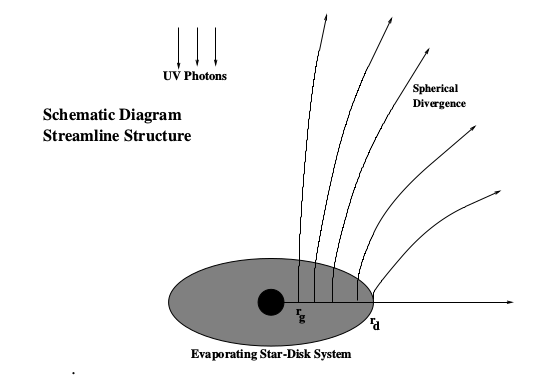
\includegraphics[width=\linewidth]{../Figures/Johnstone-1}
    \end{block}}
}
\frame{
  \twocolspic{\begin{block}{}
      The head is shaped by the incident UV radiation from the massive star, forming a D type Ionization Front, while the tail is shaped by diffuse and ionizing radiation.
    \end{block}
}{ \begin{block}{}
    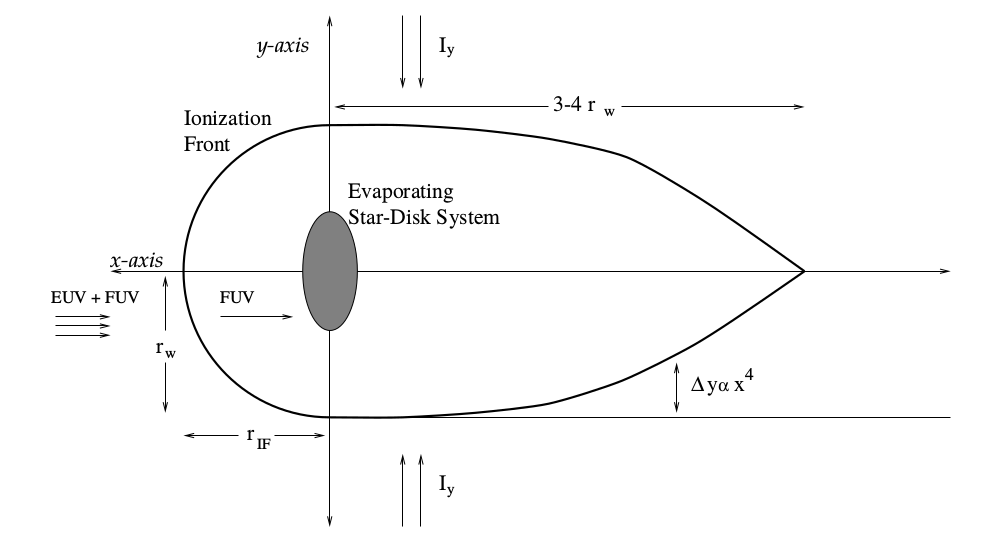
\includegraphics[width=\linewidth]{../Figures/Johnstone-shape} \\
    \citep{Johnstone:1998}
  \end{block}
  
}
}
\frame{}
\section{Fundamental Concepts}
\frame{\frametitle{General Considerations}

}
\frame{\frametitle{Planitude and Alatude}
  \small
  \twocols{\begin{block}{}
      To characterize the shape of a given bow shock we use a set of parameters:
      \begin{itemize}
      \item \textbf<2>{The radius at the apex, called $R_0$, which gives us the bow shock physical scale, and is computed as the minimum of $R(\theta)$}
      \item \textbf<3>{The assymptotic angle $\theta_\infty$ of the far wings (which usually is not measurable)}
      \item \textbf<4>{The planitude $\Pi\equiv R_c/R_0$, which measures how flat is the apex}
        \item \textbf<5>{The alatude $\Lambda\equiv R_{90}/R_0$, which measures how open the wings are}
      \end{itemize}
      
    \end{block}}{\begin{block}{}\includegraphics<1>[width=\linewidth]{../Figures/characteristic-radii}
      \includegraphics<2>[width=\linewidth]{../Figures/characteristic-radii-r0}
      \includegraphics<3>[width=\linewidth]{../Figures/characteristic-radii-thinf}
      \includegraphics<4>[width=\linewidth]{../Figures/characteristic-radii-Pi}
      \includegraphics<5>[width=\linewidth]{../Figures/characteristic-radii-Lambda}
    \end{block}}
}

\frame{\frametitle{Quadrics of Revolution}
  \twocols{\begin{block}{}
      Quadrics of Revolution are the surfaces of revolution of conic sections. May be a good and useful approximation to more complex surfaces
    \end{block}}{\begin{block}{}
      \includegraphics[width=\linewidth]{../Figures/Quadrics}
    \end{block}
  }
}

\frame{\frametitle{Quadrics of Revolution: basic definitions}
  \begin{block}{}
    Our conic section symmetry axis is aligned with the $x$ axis, and the center is displaced from the origin by distance called $x_0$. The physical scale of the conic section is set using the semi-major and semi-minor axis $a$ and $b$.
  \twocols{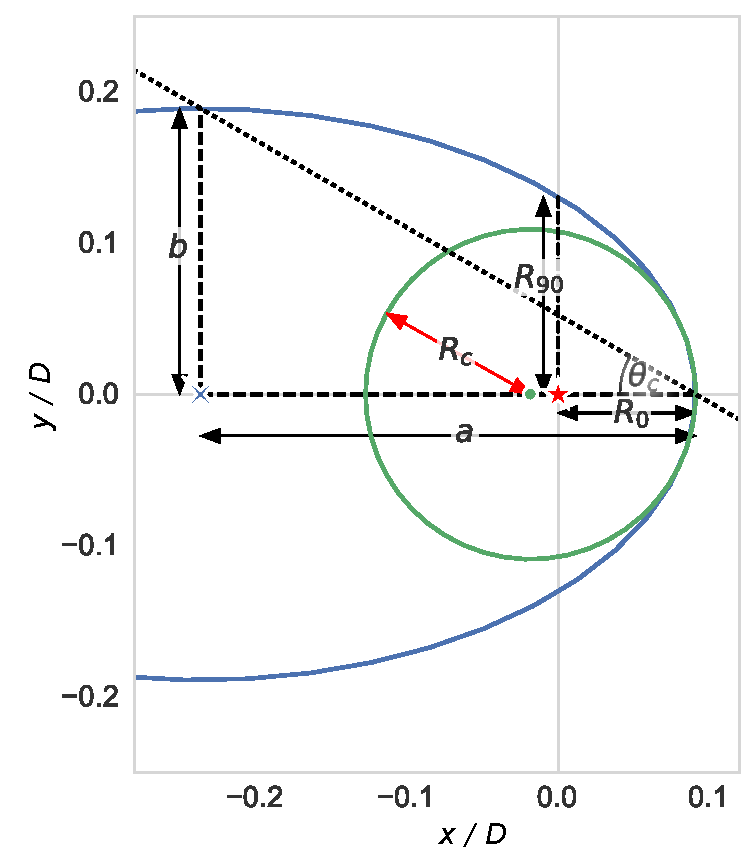
\includegraphics[width=0.7\linewidth]{../Figures/ellipse_edited}}
  {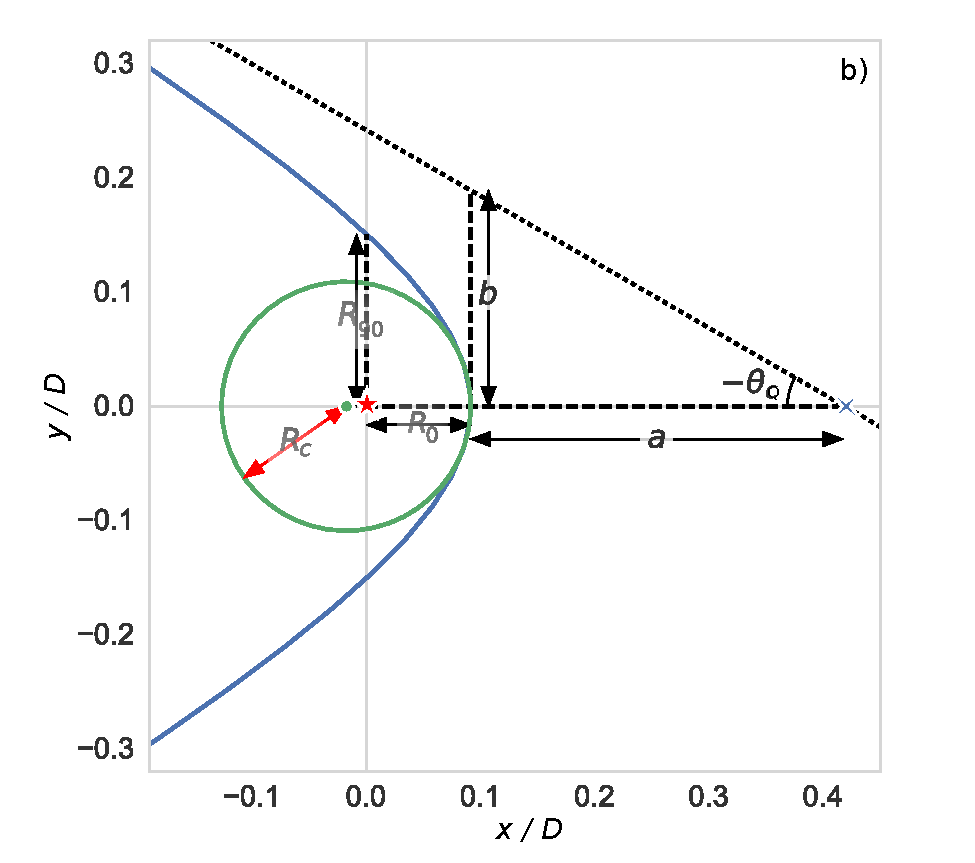
\includegraphics[width=\linewidth]{../Figures/hyperbola_edited}}
  \end{block}
}
\newcommand\Sin{\ensuremath{\mathcal{S}}}
\newcommand\Cos{\ensuremath{\mathcal{C}}}
\frame{\frametitle{Quadrics of Revolution: basic definitions}
  \twocols{\begin{block}{Parametrization}
      \footnotesize
      \begin{align}
        x &= x_0 + \sigma a\Cos(t)\\
        y &= b\Sin(t) \\
        \tan\theta &= \frac{b\Sin(t)}{x_0 + \sigma a\Cos(t)}\\
        R &= \left[\left(x_0 + \sigma a\Cos(t)\right)^2 + b^2\Sin^2(t)\right]^{1/2}
      \end{align} 
    \end{block}}{\begin{block}{where:}
      \footnotesize
      \begin{align}
        t ~&\forall~ \mathbb{R} \\
  \Cos(t), \Sin(t) &=\left\lbrace
  \begin{array}{lr}
    \cos{t}, \sin t & \mathrm{ellipses}\\
    \cosh{t}, \sinh{t} & \mathrm{hyperbolas}       
  \end{array}\right. \\
  \sigma &= \left\lbrace
  \begin{array}{lr}
    +1 & \mathrm{ellipses} \\
    -1 & \mathrm{hyperbolas}
  \end{array}\right. \\
        x_0 &= R_0 -\sigma a %\label{eq:x0}
      \end{align}
    \end{block}}
}
\newcommand\Q{\ensuremath{\mathcal{Q}}}
\frame{\frametitle{Quadrics of Revolution: basic definitions}
  \twocols{\begin{block}{}
      The eccentricity is replaced with the quadrics parameter \Q{} defined as:
      \begin{align}
        \Q = \sigma\frac{b^2}{a^2}
      \end{align}
      Or the angle $\theta_q$:
      \begin{align}
        \tan\theta_q = \sigma\frac{b}{a}
      \end{align}
      Positive values of \Q{} are associated with closed curves (i.e. ellipsoids), and $\Q \leq 0$ are associated with open curves.
    \end{block}}{\begin{block}{}
      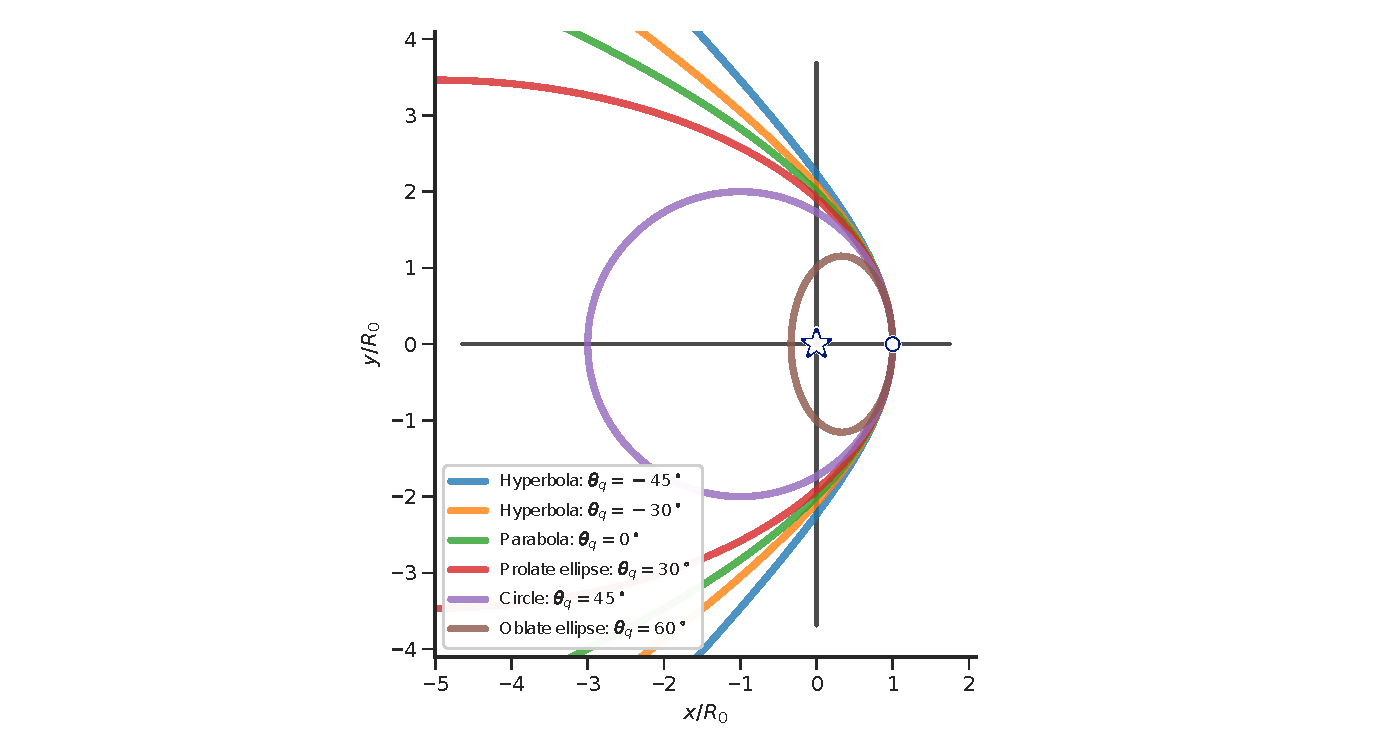
\includegraphics[width=\linewidth]{../Figures/conic1}
    \end{block}}
}
\frame{\frametitle{Quadrics of Revolution: basic definititions}
  \twocols{\begin{block}{}
      The parameters set $(a, x_0, \Q)$ is enough to characterize the curve, but for future applications the set $(R_0, \Pi, \Lambda)$ is more useful. So, the transformation between the two sets is given by:
    \end{block}}{\begin{block}{}
      \begin{align}
        R_0 &= x_0 + \sigma a \\
        \Pi &= \frac{a\Q}{a + \sigma x_0} \\
        \Lambda &= \left(\Q \frac{a - \sigma x_0}{a + \sigma x_0}\right)^{1/2}
      \end{align}
    \end{block}}
  \begin{block}{}
    Finally, the quadrics parameter (and thus the kind of quadric) may be computed from the planitude and alatude as follows:
    \begin{align}
      \Q = 2\Pi - \Lambda^2
    \end{align}
  \end{block}
  
}

\frame{\frametitle{Projection Onto the Plane of Sky}

 }
\section{Thin Shell Model}
\frame{4}
\section{Results Obtained to the Classical Proplyds of Orion Nebula}
\frame{5}
\section{Summary and Conclusions}
\frame[allowframebreaks]{\frametitle{References}
\bibliographystyle{mnras}
\bibliography{defense_biblio}
}
\end{document}

